\let\negmedspace\undefined
\let\negthickspace\undefined
\documentclass[journal,12pt,onecolumn]{IEEEtran}
\usepackage{cite}
\usepackage{amsmath,amssymb,amsfonts,amsthm}
\usepackage{algorithmic}
\usepackage{graphicx}
\graphicspath{{Figs/}}
\usepackage{textcomp}
\usepackage{xcolor}
\usepackage{txfonts}
\usepackage{listings}
\usepackage{enumitem}
\usepackage{mathtools}
\usepackage{gensymb}
\usepackage{comment}
\usepackage{caption}
\usepackage[breaklinks=true]{hyperref}
\usepackage{tkz-euclide} 
\usepackage{listings}
\usepackage{gvv}                                        
%\def\inputGnumericTable{}                                 
\usepackage[latin1]{inputenc}     
\usepackage{xparse}
\usepackage{color}                                            
\usepackage{array}                                            
\usepackage{longtable}                                       
\usepackage{calc}                                             
\usepackage{multirow}
\usepackage{multicol}
\usepackage{hhline}                                           
\usepackage{ifthen}                                           
\usepackage{lscape}
\usepackage{tabularx}
\usepackage{array}
\usepackage{float}
%\newtheorem{theorem}{Theorem}[section]
%\newtheorem{theorem}{Theorem}[section]
%\newtheorem{problem}{Problem}
%\newtheorem{proposition}{Proposition}[section]
%\newtheorem{lemma}{Lemma}[section]
%\newtheorem{corollary}[theorem]{Corollary}
%\newtheorem{example}{Example}[section]
%\newtheorem{definition}[problem]{Definition}

\begin{document}

\title{1.2.3}
\author{AI25BTECH11002 - Ayush Sunil Labhade}
{\let\newpage\relax\maketitle}
%\renewcommand{\thefigure}{\theenumi}
%\renewcommand{\thetable}{\theenumi}
Question:\newline
Find the sum of the vectors $\vec{a}= \hat{\imath}-2\hat{\jmath}+\hat{k}$, $\vec{b}= -2\hat{\imath}+4\hat{\jmath}+5\hat{k}$, $\vec{c}=\hat{\imath}-6\hat{\jmath}-7\hat{k}$. \\
\textbf{Solution:}
Given:
\begin{table}[H]
	\centering
	\begin{tabular}{|c|c|}
\hline
Point & Vector \\
\hline
$\vec{a}$ & $\myvec{1 \\ -2 \\ 1}$ \\
\hline
$\vec{b}$ & $\myvec{-2 \\ 4 \\ 5}$ \\
\hline
$\vec{c}$ & $\myvec{1 \\ -6 \\ -7}$ \\
\hline
\end{tabular}

	\label{}
	\caption{Given data}
\end{table}
\begin{align}
	\vec{r}=\brak{\vec{a}+\vec{b}+\vec{c}}
\end{align}
Substituting values,\\
\begin{align}
	\vec{r}= \myvec{0 \\ -4 \\ -1}
\end{align}
\begin{figure}[H]
	\centering
	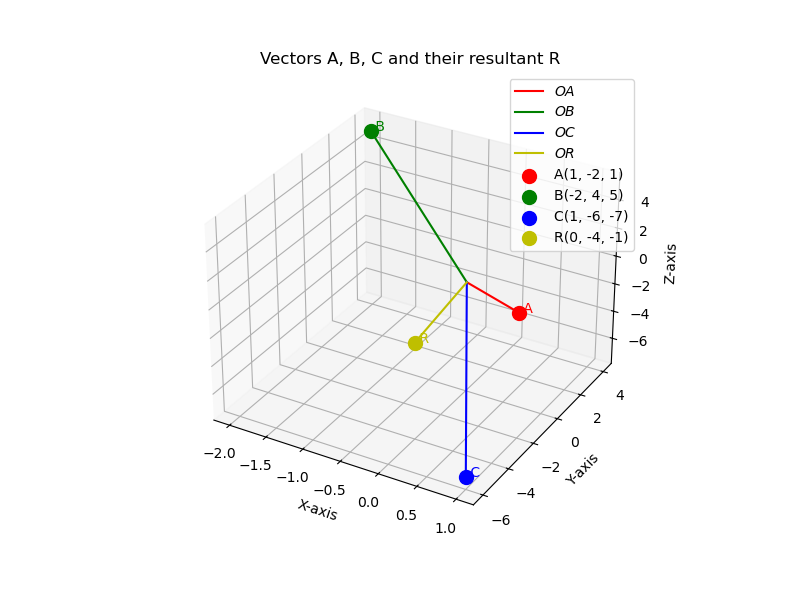
\includegraphics[scale=0.5]{plot}
	\caption*{}
	\label{fig}
\end{figure}
\end{document}
